\subsection{Evaluating \benchmark Solutions on a Real Robot}
% Demonstrating realism
\label{sec:sim2real}

\begin{figure}[t!]
    \centering
    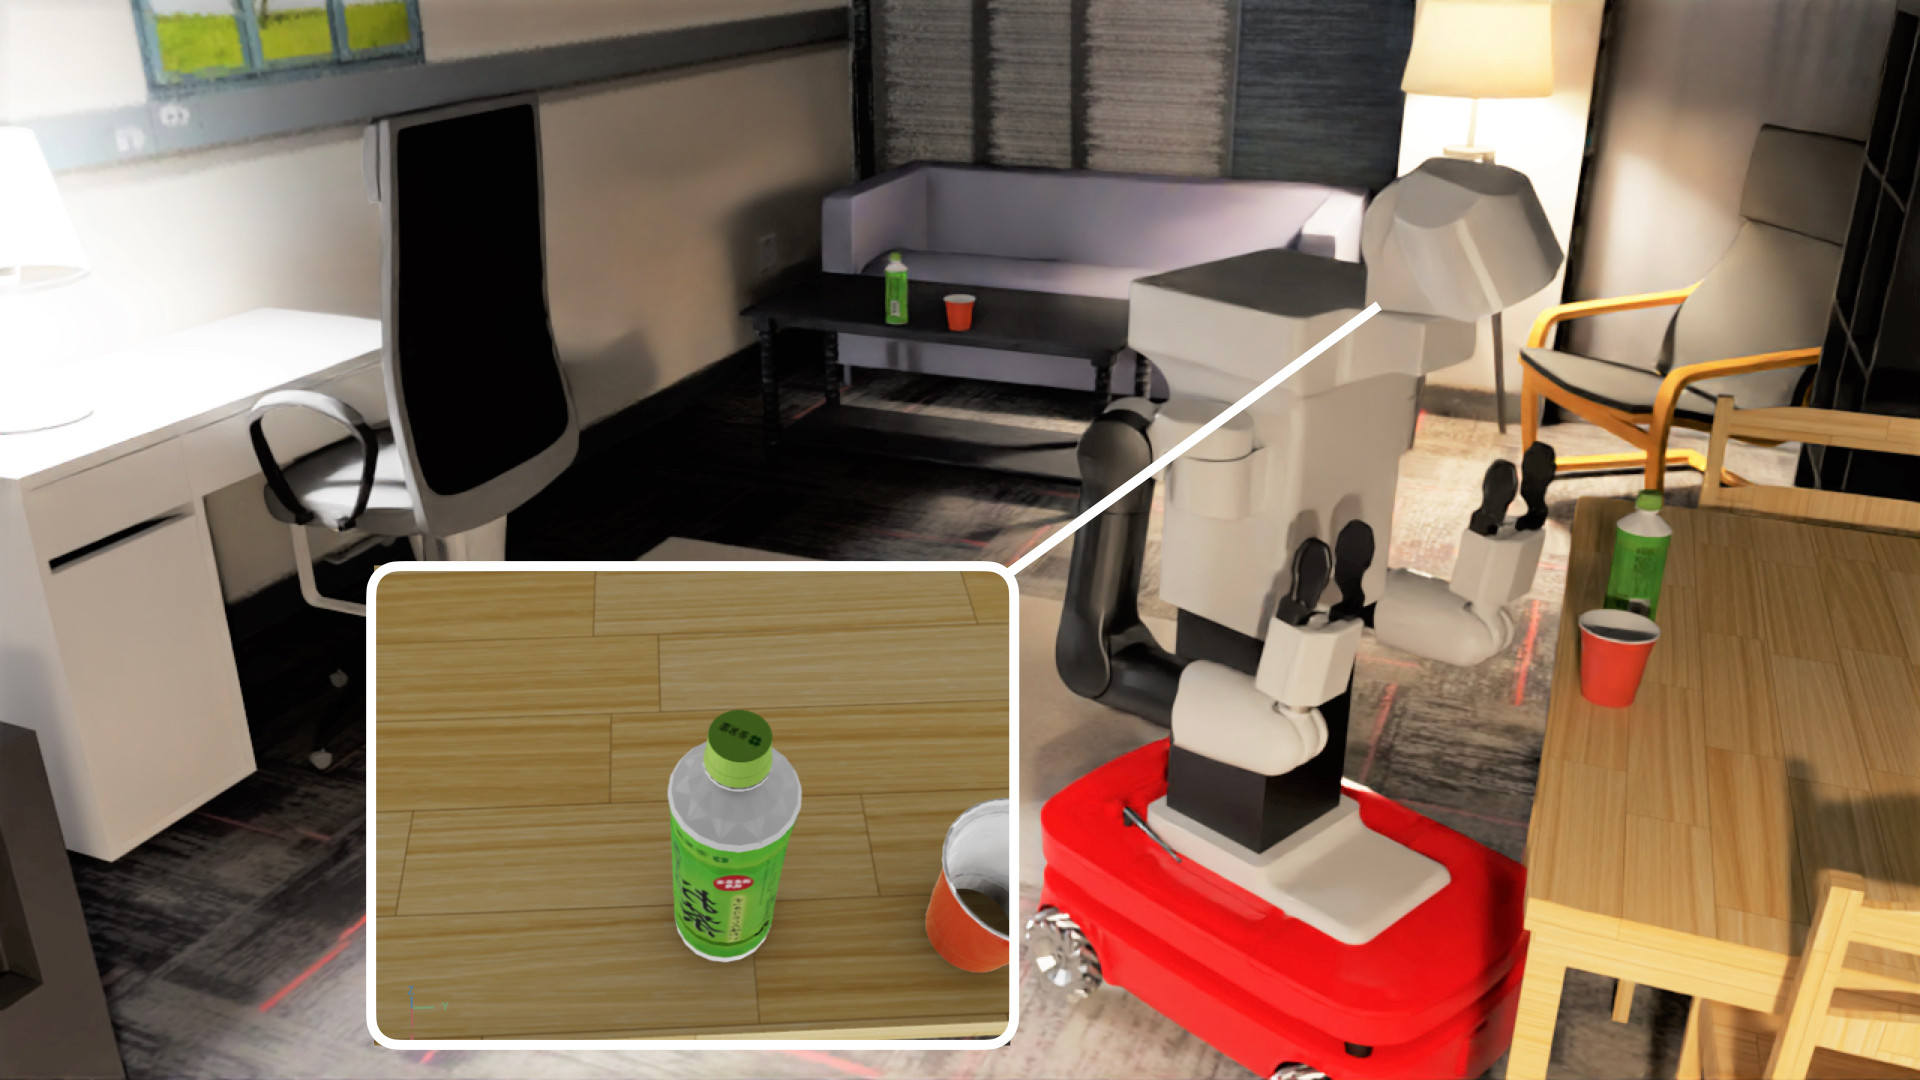
\includegraphics[width=0.27\textwidth,valign=c]{figures/sim2real/sim.001.jpeg}
    \hfill
    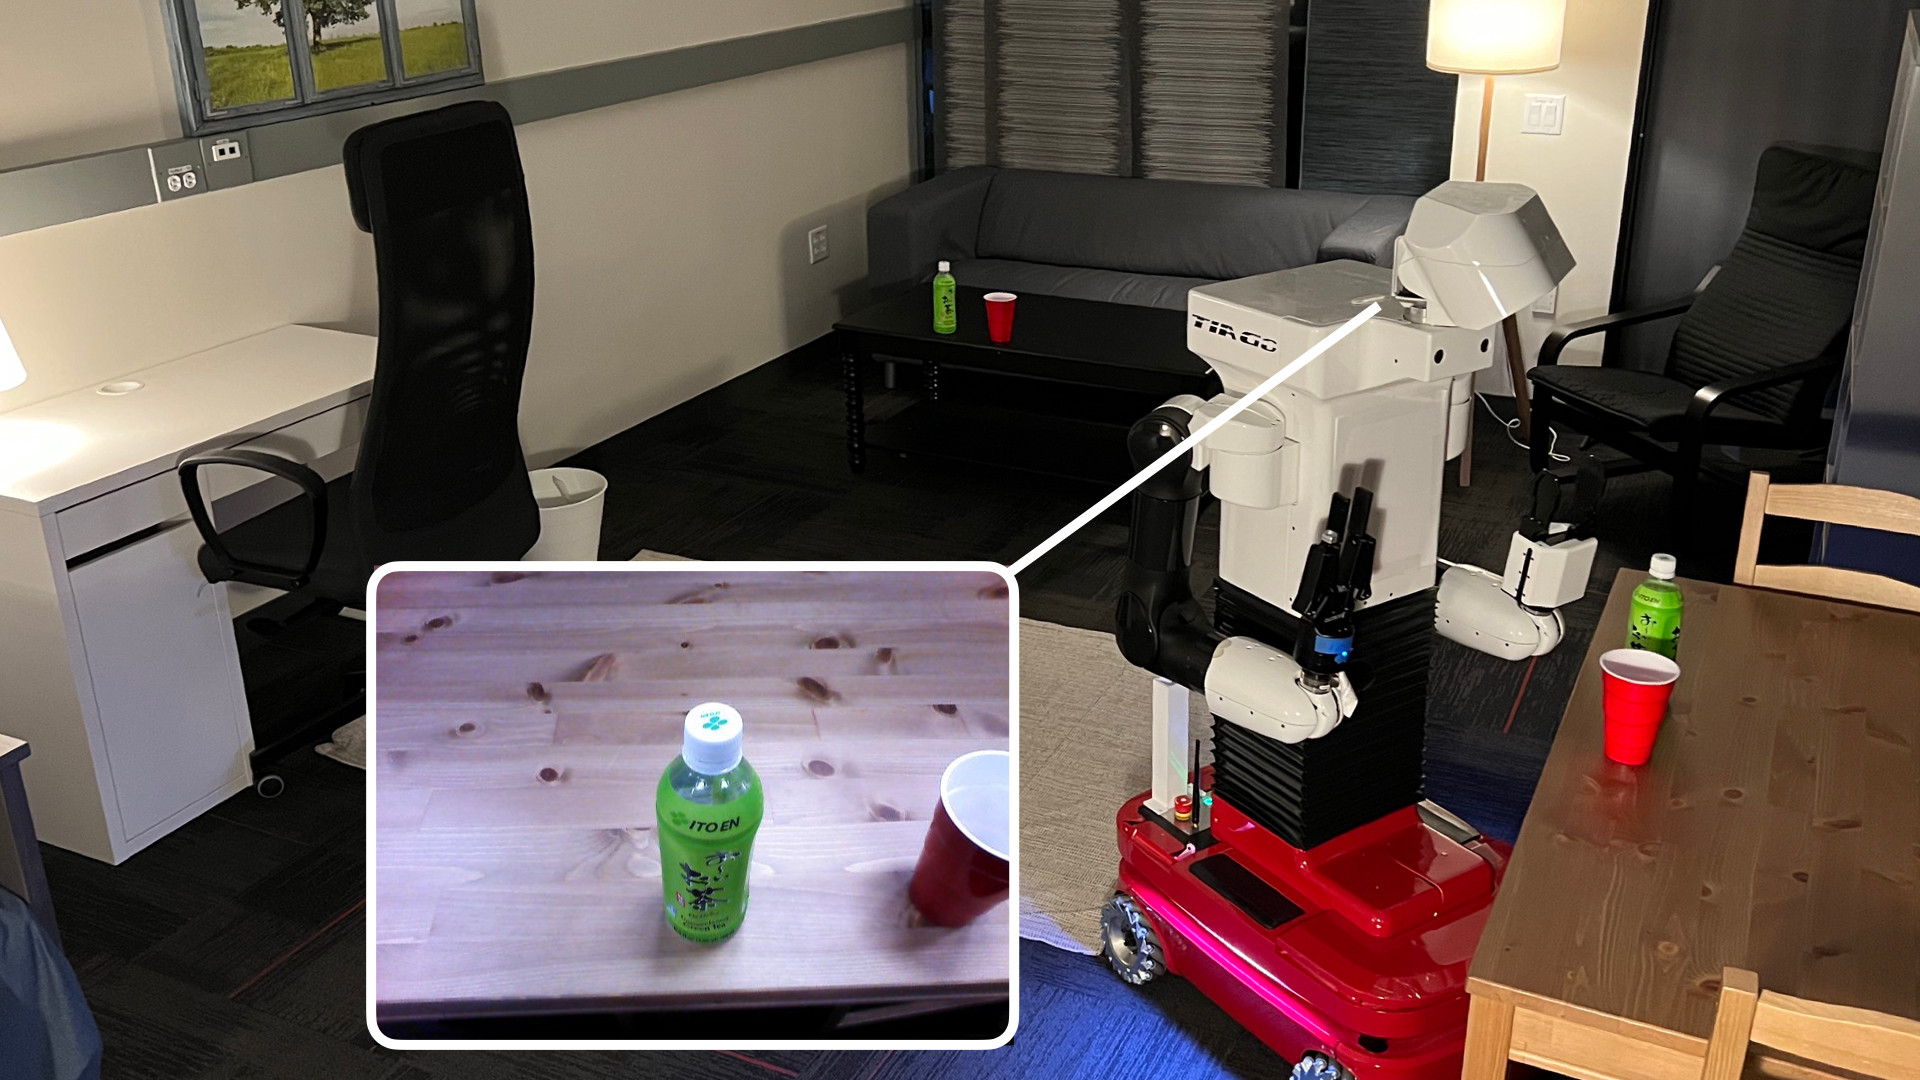
\includegraphics[width=0.27\textwidth,valign=c]{figures/sim2real/real.001.jpeg}
    \hfill
    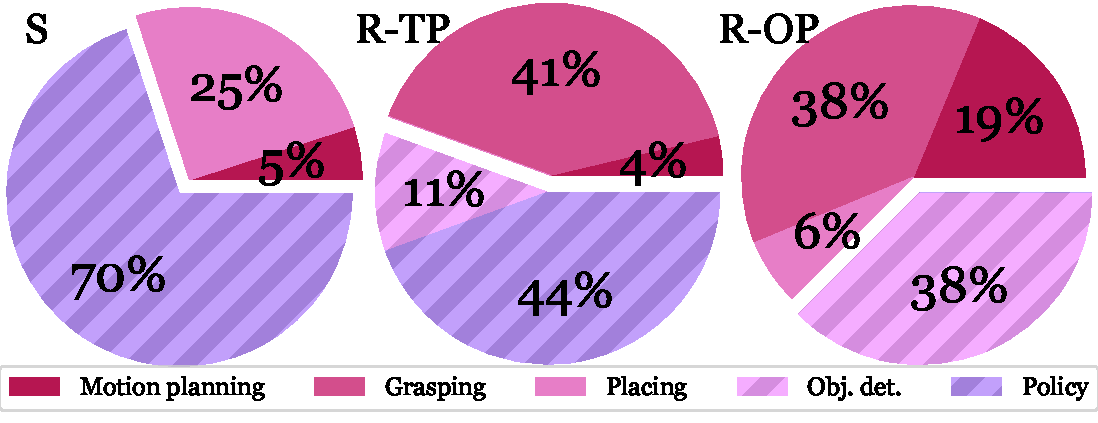
\includegraphics[width=0.44\textwidth,valign=c]{figures/sim2real/error_plot.pdf}
    \caption{\textbf{Characterizing the Sim-Real Gap:} Left: a side-by-side comparison of the simulated and the real scene, including virtual and real images obtained by the robot. While the high-resolution images are extremely similar, the mismatch in wooden texture and camera properties causes a sizable gap in the visual input to the agent. Right: source of failure in \texttt{S}imulation (\texttt{S}, left) and in \texttt{R}eal-world with a \texttt{T}rained \texttt{P}olicy in \simulator (\texttt{R-TP}, middle) and an \texttt{O}ptimal \texttt{P}olicy (\texttt{R-OP}, right) due to actuation (solid color) or perception (striped). In simulation, without full simulation of grasping (see Sec.~\ref{ss:ev_in_sim}), policy failures (i.e., selecting the wrong action primitive) dominate. On the real robot, grasping is one of the main causes of error, as well as perception issues (policy errors with the trained visual policy, object detection errors with the optimal policy).}
    \label{fig:sim2real_setup}
\end{figure}

% One of the main advantages of B1K on OmniGibson is the high level of realism (in virtual images, in physics, in distribution and quality of the assets, in the definition of activities). This realism should facilitate the ultimate goal of our benchmark: creating solutions that can transfer to real-world tasks. 

We performed a series of experiments with a real robot to answer the question: \textit{what are the main sources of discrepancy between our realistic simulation and the real world?}
To that end, we used a real-world counterpart of the simulated scene of a mockup apartment for the \texttt{CollectTrash} activity. We scanned the apartment and converted it into a virtual, interactive scene. % digital twin of this apartment in our lab, created by first 3D scanning, then replacing walls, floors, ceilings and all objects by 3D models from our dataset.
We use a real bi-manual mobile manipulator Tiago, and leverage the RGB-D images from its onboard sensors and a YOLOv3 object detector~\cite{redmon2018yolov3,bjelonicYolo2018} to localize the objects in 3D space for manipulation. 
For navigation, the robot localizes with a particle filter~\cite{thrun2005probabilistic} based on two LiDAR sensors and a map of the apartment.
% We query the location of the objects using the area of depth channel of the RGB-D camera that corresponds to the bounding box detection.
The action primitives are implemented with the same sampling-based motion planning algorithm as in simulation~\cite{kuffner2000rrt,Jordan.Perez.ea:CSAIL13} with additional tuning. 
% e study the sim2real transference of a solution for \texttt{collect\_trash} to a real robot. Our goal is to assess the potential differences in perception and execution between the real robot actuation/sensing and the simulated one.
% We transfer the most successful policy trained in simulation, the RL policy using action primitives (see Sec.~\ref{} and Table~\ref{}). The locations where to collect bottles and cups to place them are the same as in simulation, and defined in the registered 2D map used for real-robot localization. However, we do not assume that the object location is known. We integrate an object detector based on YOLO~\ref{} that provides bounding boxes around the objects of interest. The 3D location of the objects, used to parameterize actions such as \texttt{grasping} and \texttt{placing}, is obtained from the area of the depth image corresponding to the detection bounding box. The action primitives are solved using the same sampling-based motion planning algorithm as in simulation. 
% Considering a successful trial only when all four trash items are successfully gathered into the trash bin, our solution achieves XXX success, indicating that the realism of B1K in OmniGibson makes direct sim2real transfer possible. However, this is a drop in performance wrt. the success rate of the same solution in simulation (XXX\%).
We evaluate two strategies for selecting action primitives in the real world: an optimal policy based on human input, and a vision-based policy (\rlprim) trained in \simulator. To facilitate sim-to-real transfer, during training we additionally applied image-based data augmentation to the observations based on a prior work~\cite{fan2021secant} (see Appendix~\ref{as:s2r} for further details). With the optimal policy, we evaluate the gap in actuation between the simulated and the real robot; with the learned policy, we also evaluate the gap in visual perception. We achieve different success rates in simulation (50 runs, $\sim$40\% success) and in the real world with optimal (27 runs, $\sim$22\%) and trained policies (26 runs, 0\%), hinting at a sim-real gap that we analyze below.
%Note that in simulation, we evaluate with assistive \textit{Pick} primitive because our previous analysis (Sec.~\ref{ss:ev_in_sim}) shows that physics-based grasping has a significant adverse effect on performance - indicating the difficulty of simulating realistic grasping.%  that failures in execution with fully simulated grasping would be caused 100\% of the time by grasping.

The failure cases are depicted in Fig.~\ref{fig:sim2real_setup} (right). We observe that the majority of failures in simulation are due to the visual policy (perception), while others are caused by stochasticity in the \texttt{place} primitive and the sampling-based motion planner. The reason why none of the failures are due to grasping is that, in simulation, we evaluate with the assistive \texttt{pick} primitive. %, as physics-based grasping would significantly degrade the policy performance (Sec.~\ref{ss:ev_in_sim}), highlighting the difficulty of training reinforcement learning agents with physically realistic grasping.
Grasping is fairly difficult in the real world, contributing to around 40\% of the failures for both the trained and the optimal policy. %the main failure case in the real world is unsuccessful grasping. It is also important to note that not all errors in the real world are caused by grasping, indicating a mismatch in the difficulty of grasping in simulation and in the real world.
For the learned policy, 44\% of the errors come from the visual policy selecting the wrong action primitive due to the differences between the simulated and the real images. The visual discrepancy results from unmodeled effects such as the real camera's poor dynamic range (see Fig.~\ref{fig:sim2real_setup}, left and middle) % and contrast between the ASUS camera and the virtual camera, where the simulated camera does not accurately reproduce the dynamic range of the real camera. 
and imperfect object modeling (e.g. the exact wooden texture and the surface reflectivity of the tables), which can be alleviated by more targeted domain randomization.
Interestingly, several manipulation failures on the real robot are caused by unfavorable robot base placement resulting from navigation inaccuracies in the previous timestep. This compounding source of error is not present in simulation because we assume perfect localization and execution. %navigation is unrealistically accurate.

We believe this analysis provides relevant information about the main sources and severity of the sim-real gap in \benchmark in \simulator, and provide insights for future research avenues.
Our plan is to use some of these insights to create novel sim-to-real solutions that make progress on \benchmark.
% Fig.~\ref{fig:sim2real_results} depict a further analysis of the differences. We see that the few failures in simulation are caused by XXX (xxx failures). Differently, most failures in simulation are caused by XXX (xxx failures) and XXX (xxx failures). XXX is also a significant harder challenge in real-world than in simulation. These are avenues of improvement for simulators and for novel research that can facilitate sim2real transfer. Further analysis and comparisons between simulation and real can be found in our Appendix.



% \begin{figure}[t!]
%     \centering
%     \includegraphics[width=0.45\textwidth]{figures/sim2real/comparison_sim2realb.jpg}
%     \includegraphics[width=0.4\textwidth]{figures/sim2real/reasons_sim2real2.jpg}
%     \caption{[In main body of text] Left: degree of completion (Q) of our solution in simulation and in real-world: while the direct sim2real transfer achieves some success, it is only able to fulfill the entire task (collect four objects) in XXX of the trials. Right: analysis of the causes of failure in simulation and in real-world: the few failures in simulation are caused by XXX. On the real robot, the noise in actuation and in sensing is XXXX}
%     \label{fig:sim2real_results}
% \end{figure}

%Optional if we have time: YOLO experiments on real scenes and virtual scenes. 